\chapter{Applications}

\fbox{
    \parbox{\textwidth}
    {
        Architecture guidelines for stable Deep Convolutional GANs
        \begin{itemize}
            \item Replace any pooling layers with strided convolutions (discriminator) and fractional-strided convolutions (generator).
            \item Use batchnorm in both the generator and the discriminator.
            \item Remove fully connected hidden layers for deeper architectures.
            \item Use ReLU activation in generator for all layers except for the output, which uses Tanh.
            \item Use LeakyReLU activation in the discriminator for all layers.
        \end{itemize}
    }
}

\pagebreak



\section{BayesCNN for Image Super Resolution}

The task referred as Super Resolution is the recovery of a High Resolution image from a given Low Resolution image. It is applicable to many areas like medical imaging \citet{10.1007/978-3-642-40760-4_2}, face recognition \citet{1203152} and so on.

There are many ways to do a single image super resolution and a detailed benchmarks of the methods is provided by Yang \citet{Yang2014SingleImageSA}. Following are the major ways to do a single image super resolution:\\
Prediction Models. SISR algorithms in this category generate HR images
from LR inputs through a predefined mathematical formula without training
data. Interpolation-based methods (bilinear, bicubic, and Lanczos) generate HR pixel intensities by weighted averaging neighboring LR pixel values. Since interpolated intensities are locally similar to neighboring pixels, these algorithms generate good smooth regions but insufficient large gradients along edges and at high-frequency regions. The IP method [16] exploits a predefined downsampling model from a HR image to a LR image. Given an initial HR image, this method iteratively generates a LR image through the predefined downsampling model and compensates the difference map in LR back to the HR image. Since a generated HR image is designed to best match the LR input image under the linear downsampling model, the contrast along edges is better enhanced than the results generated by bicubic interpolation.\\

Edge Based Methods. Edges are important primitive image structures that
play a prime role in visual perception. Several SISR algorithms have been proposed to learn priors from edge features for reconstructing HR images. Various edge features have been proposed such as the depth and width of an edge [8] or the parameter of a gradient profile [30]. Since the priors are primarily learned from edges, the reconstructed HR images have high-quality edges with proper sharpness and limited artifacts. However, edge priors are less effective for modeling other high-frequency structures such as textures.\\

Patch Based Methods. Given a set of paired LR and HR training images,
patches can be cropped from the training images to learn mapping functions.]. In addition to equally averaging overlapped patches, several methods for blending overlapped pixels have been proposed including weighted averaging [11,44], Markov Random Fields [10], and Conditional Random Fields [38].



The global \ac{SR} problem assumes \ac{LR} data to be a low-pass filtered (blurred), downsampled and noisy version of \ac{HR} data. It is a highly ill-posed problem, due to the loss of high-frequency information that occurs during the non-invertible low-pass filtering and subsampling operations. Furthermore, the SR operation is effectively a one-to-many mapping from \ac{LR} to \ac{HR} space which can have multiple solutions, of which determining the correct solution is non-trivial. A key assumption that underlies many \ac{SR} techniques is that much of the high-frequency data is redundant and thus can be accurately reconstructed from low frequency components. \ac{SR} is therefore an inference problem, and thus relies on our model of the statistics of images in question.


\subsection{Our Approach}

We build our work upon \citet{DBLP:journals/corr/ShiCHTABRW16} work that shows that performing Super Resolution work in High Resolution space is not the optimal solution and it adds the computation complexity. We used a Bayesian Convolutional Neural Network to extract features in the Low Resolution space. We use an efficient sub-pixel convolution layer, as proposed by \citet{DBLP:journals/corr/ShiCHTABRW16}, which learns an array of upscaling filters to upscale the final Low Resolution feature maps into the High Resolution output. This replaces the handcrafted bicubic filter in the Super Resolution pipeline with more complex upscaling filters specifically trained for each feature map, and also reduces the computational complexity of the overall Super Resolution operation.

\begin{figure*}[htbp]
\begin{center}
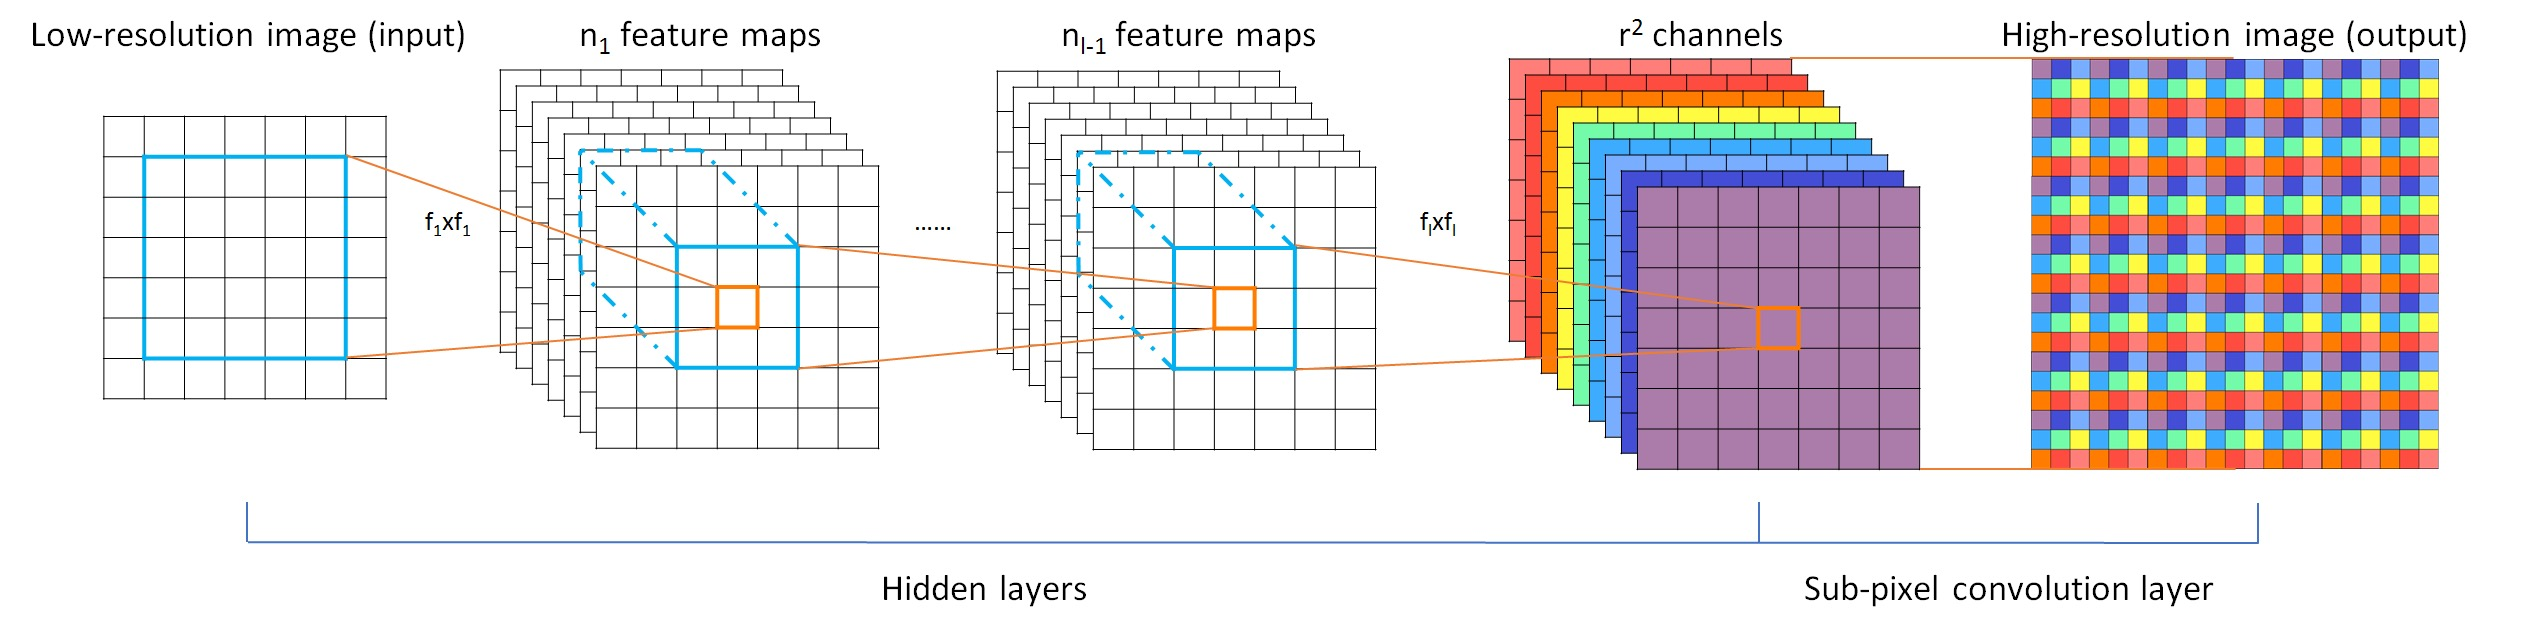
\includegraphics[width=1.0\linewidth]{Chapter6/Figs/networkstructure.jpg}
\caption{The proposed efficient sub-pixel convolutional neural network (ESPCN), with two convolution layers for feature maps extraction, and a sub-pixel convolution layer that aggregates the feature maps from \ac{LR} space and builds the \ac{SR} image in a single step.}
\label{fig:networkstructure}
\end{center}
\end{figure*}

\subsection{Empirical Analysis}



\section{BayesCNN for Generative Adversarial Networks}

Generative Adversarial Networks (GANs) \cite{goodfellow2014generative} can be used for two major tasks: to learn good feature representations by using the generator and discriminator networks as feature extractors, and to generate natural images. The learned feature representation or generated images can reduce the number of images substantially for a computer vision supervised task. However GANs were quite unstable to train in the past and that is why we base our work on the stable GAN architecture namely Deep Convolutional GANs (DCGAN) \cite{DBLP:journals/corr/RadfordMC15}. We use the trained Bayesian discriminators for image classification tasks, showing competitive performance with the normal DCGAN architecture.

\subsection{Our approach}
\subsection{Empirical Analysis}



